\documentclass[11pt]{article}
\usepackage[utf8]{inputenc}
\usepackage[T1]{fontenc}
\usepackage[spanish]{babel}
\usepackage{amsmath, amssymb, amsthm, mathtools}
\usepackage{braket}
\usepackage{dsfont}
\usepackage{graphicx}
\usepackage[margin=2.5cm]{geometry}
\usepackage{hyperref}

\newcommand{\ii}{\mathrm{i}}
\newcommand{\ee}{\mathrm{e}}
\newcommand{\adag}{\hat a^\dagger}
\newcommand{\Tr}{\operatorname{Tr}}
\newcommand{\Real}{\operatorname{Re}}

\title{Preparaci\'on de estados y entrelazamiento}
\author{Ricardo Del Rosal Gardu\~no \\ \small Doctorado en F\'isica, BUAP}
\date{Notas a partir de Schleich, \emph{Quantum Optics in Phase Space}}

\begin{document}
\maketitle

\tableofcontents
\bigskip

\section{Idea f\'isica}

Despu\'es de la interacci\'on de Jaynes-Cummings-Paul, el estado del \'atomo y
el estado del campo ya no tienen por qu\'e factorizarse. En general no existe
una escritura de la forma
\begin{equation}
  \ket{\psi(t)}
  =
  \ket{\psi_{\mathrm{at}}(t)}
  \otimes
  \ket{\psi_{\mathrm{c}}(t)} .
\end{equation}
Cuando esto ocurre, el \'atomo y el campo est\'an entrelazados. La informaci\'on
sobre el campo queda parcialmente escrita en los grados de libertad internos
del \'atomo, y la informaci\'on sobre el \'atomo queda parcialmente escrita en
el campo. Por eso, midiendo el \'atomo se puede obtener informaci\'on del campo
de radiaci\'on. M\'as a\'un, si despu\'es de la interacci\'on se selecciona
\'unicamente cierto resultado at\'omico, la medici\'on no solo observa el campo:
tambi\'en lo prepara. Esta es la idea b\'asica de la ingenier\'ia de estados
cu\'anticos.

Se toma como punto de partida el ansatz general
\begin{equation}
  \ket{\psi(t)}
  =
  \sum_{n=0}^{\infty}
  \left(
  \psi_{a,n}(t)\ket{a,n}
  +
  \psi_{b,n}(t)\ket{b,n}
  \right),
\end{equation}
donde $\ket{a}$ es el estado at\'omico excitado, $\ket{b}$ el estado base y
$\ket{n}$ el estado de Fock del campo. Todas las probabilidades de medici\'on
se obtienen proyectando este vector sobre el estado de referencia adecuado.

\section{Medici\'on conjunta \'atomo-campo}

Se prepara inicialmente el \'atomo en un estado $\ket{\psi_{\mathrm{at}}(0)}$
y el campo en $\ket{\psi_{\mathrm{c}}(0)}$. Despu\'es se dejan interactuar
durante un tiempo $t$. Al final se pregunta si el \'atomo se encuentra en un
estado de referencia $\ket{F_{\mathrm{at}}}$ y si el campo se encuentra en un
estado de referencia $\ket{F_{\mathrm{c}}}$. Cuando ambos subsistemas se
encuentran en sus estados de referencia, el evento se acepta; si no, se
descarta.

La mec\'anica cu\'antica no predice un resultado individual con certeza. Lo que
predice es la probabilidad de obtener ese resultado. Para una medici\'on
conjunta, la amplitud de probabilidad es
\begin{equation}
  A(t;F_{\mathrm{at}},F_{\mathrm{c}})
  =
  \bra{F_{\mathrm{c}}}\bra{F_{\mathrm{at}}}\psi(t)\rangle,
\end{equation}
y la probabilidad asociada es
\begin{equation}
  \boxed{
  W(t;F_{\mathrm{at}},F_{\mathrm{c}})
  =
  \left|
  \bra{F_{\mathrm{c}}}\bra{F_{\mathrm{at}}}\psi(t)\rangle
  \right|^2 .
  }
\end{equation}
Sustituyendo el ansatz,
\begin{align}
  A(t;F_{\mathrm{at}},F_{\mathrm{c}})
  =
  \sum_{n=0}^{\infty}
  \big[
  &\psi_{a,n}(t)
  \braket{F_{\mathrm{at}}|a}
  \braket{F_{\mathrm{c}}|n}
  \notag\\
  &+
  \psi_{b,n}(t)
  \braket{F_{\mathrm{at}}|b}
  \braket{F_{\mathrm{c}}|n}
  \big].
\end{align}
Es importante que primero se suman amplitudes y solamente despu\'es se toma el
m\'odulo cuadrado. Por tanto, si el estado de referencia del campo tiene
superposici\'on de varios n\'umeros de fotones, las contribuciones con
distintos $n$ interfieren entre s\'i. Esta interferencia no es un detalle
algebraico: es la se\~nal de que la medici\'on conjunta conserva informaci\'on
de fase entre los distintos caminos cu\'anticos que llevan al mismo resultado
final.

\section{Medici\'on del estado interno del \'atomo}

Si \'unicamente se mide el estado interno del \'atomo y no se observa en qu\'e
estado qued\'o el campo, entonces el campo debe tratarse como grado de libertad
no observado. Matem\'aticamente esto significa sumar sobre una base completa
del campo. Usando la base de Fock,
\begin{equation}
  \boxed{
  W(t;F_{\mathrm{at}})
  =
  \sum_{n=0}^{\infty}
  \left|
  \bra{n}\bra{F_{\mathrm{at}}}\psi(t)\rangle
  \right|^2 .
  }
\end{equation}
Si el estado de referencia at\'omico es
\begin{equation}
  \ket{F_{\mathrm{at}}}=f_a\ket{a}+f_b\ket{b},
\end{equation}
entonces
\begin{equation}
  \bra{n}\bra{F_{\mathrm{at}}}\psi(t)\rangle
  =
  f_a^*\,\psi_{a,n}(t)
  +
  f_b^*\,\psi_{b,n}(t),
\end{equation}
y, por tanto,
\begin{equation}
  W(t;F_{\mathrm{at}})
  =
  \sum_{n=0}^{\infty}
  \left|
  f_a^*\,\psi_{a,n}(t)
  +
  f_b^*\,\psi_{b,n}(t)
  \right|^2 .
\end{equation}
Para los dos estados internos de la base at\'omica se recuperan las
poblaciones usuales:
\begin{equation}
  W(t;a)=\sum_{n=0}^{\infty}|\psi_{a,n}(t)|^2,
  \qquad
  W(t;b)=\sum_{n=0}^{\infty}|\psi_{b,n}(t)|^2.
\end{equation}

La diferencia con la medici\'on conjunta es conceptual. En la medici\'on
conjunta se proyecta tambi\'en el campo sobre un estado definido y sobreviven
interferencias entre diferentes n\'umeros de fotones. En la medici\'on
at\'omica marginal, en cambio, se suma incoherentemente sobre los estados del
campo: cada valor de $n$ contribuye con una probabilidad, no con una amplitud
com\'un con los dem\'as valores de $n$.

Al expandir el m\'odulo cuadrado, para cada $n$ aparecen t\'erminos diagonales,
\begin{equation}
  |f_a|^2|\psi_{a,n}|^2
  +
  |f_b|^2|\psi_{b,n}|^2,
\end{equation}
que son reales y no negativos, y t\'erminos cruzados,
\begin{equation}
  f_a^*f_b\,\psi_{a,n}\psi_{b,n}^*
  +
  f_b^*f_a\,\psi_{b,n}\psi_{a,n}^*,
\end{equation}
que dependen de la fase relativa entre las amplitudes at\'omicas. Esos
t\'erminos cruzados pueden sumar o restar y son los responsables de la
interferencia cuando el estado de referencia at\'omico es una superposici\'on.

\section{Medici\'on del estado del campo}

Si se mide el campo en un estado $\ket{F_{\mathrm{c}}}$ y no se observa el
estado at\'omico, entonces se traza sobre los dos estados internos del \'atomo:
\begin{equation}
  \boxed{
  W(t;F_{\mathrm{c}})
  =
  \sum_{s=a,b}
  \left|
  \bra{F_{\mathrm{c}}}\bra{s}\psi(t)\rangle
  \right|^2 .
  }
\end{equation}
En t\'erminos de probabilidades conjuntas,
\begin{equation}
  W(t;F_{\mathrm{c}})
  =
  W(t;a,F_{\mathrm{c}})
  +
  W(t;b,F_{\mathrm{c}}).
\end{equation}
La suma es incoherente entre los resultados at\'omicos $a$ y $b$ porque esos
resultados son distinguibles. Si no se lee el \'atomo, pero en principio el
estado at\'omico contiene informaci\'on sobre el camino seguido por el sistema,
esa informaci\'on reduce las interferencias visibles en el campo reducido.

\section{Estados condicionales tras la medici\'on}

Si se detecta el \'atomo en el estado $\ket{F_{\mathrm{at}}}$, el estado del
campo se obtiene proyectando el estado total sobre ese estado at\'omico:
\begin{equation}
  \ket{\tilde\psi_{\mathrm{c}}(t;F_{\mathrm{at}})}
  =
  \bra{F_{\mathrm{at}}}\psi(t)\rangle .
\end{equation}
La tilde recuerda que este vector no est\'a normalizado. Su norma cuadrada es
precisamente la probabilidad de obtener el resultado at\'omico:
\begin{equation}
  \braket{\tilde\psi_{\mathrm{c}}|\tilde\psi_{\mathrm{c}}}
  =
  W(t;F_{\mathrm{at}}).
\end{equation}
Por tanto, el estado normalizado del campo condicionado a esa detecci\'on es
\begin{equation}
  \boxed{
  \ket{\psi_{\mathrm{c}}(t;F_{\mathrm{at}})}
  =
  \frac{
  \bra{F_{\mathrm{at}}}\psi(t)\rangle
  }{
  \sqrt{W(t;F_{\mathrm{at}})}
  } .
  }
\end{equation}
El significado f\'isico es directo: este estado del campo solo aparece en las
corridas donde el \'atomo fue encontrado en $\ket{F_{\mathrm{at}}}$. Como ese
evento ocurre con probabilidad $W(t;F_{\mathrm{at}})$, la normalizaci\'on debe
hacerse con esa misma probabilidad.

De forma an\'aloga, si se mide el campo en $\ket{F_{\mathrm{c}}}$, el estado
at\'omico condicionado queda
\begin{equation}
  \boxed{
  \ket{\psi_{\mathrm{at}}(t;F_{\mathrm{c}})}
  =
  \frac{
  \bra{F_{\mathrm{c}}}\psi(t)\rangle
  }{
  \sqrt{W(t;F_{\mathrm{c}})}
  } .
  }
\end{equation}

\section{Medici\'on experimental del \'atomo}

\subsection{Medici\'on de poblaciones por ionizaci\'on}

Para medir si el \'atomo sali\'o en $\ket{a}$ o en $\ket{b}$ se usa
t\'ipicamente ionizaci\'on selectiva por campo el\'ectrico. Se aplica un campo
externo en la direcci\'on $z$,
\begin{equation}
  \mathbf E=E_0\,\hat{\mathbf z},
\end{equation}
de modo que la energ\'ia potencial asociada al dipolo en el campo externo es
\begin{equation}
  V_E(z)=-\mathbf d\cdot\mathbf E.
\end{equation}
Para un electr\'on ligado, esta contribuci\'on inclina el potencial
Coulombiano. De manera esquem\'atica,
\begin{equation}
  V_{\mathrm{tot}}(z)
  =
  V_C(z)+V_E(z)
  \simeq
  -\frac{e^2}{4\pi\epsilon_0|z|}
  -
  eE_0 z,
\end{equation}
con el signo efectivo fijado por la direcci\'on del campo y la carga del
electr\'on. Al aumentar $E_0$, la barrera de potencial se reduce. Un estado de
Rydberg con energ\'ia m\'as alta puede tunelar e ionizarse para un campo m\'as
d\'ebil que un estado m\'as ligado. As\'i, si los niveles $\ket{a}$ y
$\ket{b}$ tienen umbrales de ionizaci\'on distintos, se incrementa el campo
el\'ectrico en el tiempo y se observa la corriente de ionizaci\'on $I(t)$.

La posici\'on temporal de los m\'aximos de $I(t)$ indica qu\'e nivel se
ioniz\'o, y el \'area bajo cada m\'aximo da informaci\'on sobre la poblaci\'on
correspondiente. De esta forma se miden directamente las probabilidades
$W(t;a)$ y $W(t;b)$.

\subsection{Proyecci\'on sobre superposiciones at\'omicas}

La ionizaci\'on selectiva mide poblaciones en la base $\{\ket{a},\ket{b}\}$.
Para medir una superposici\'on arbitraria,
\begin{equation}
  \ket{F_{\mathrm{at}}}
  =
  \epsilon_a\ket{a}
  +
  \epsilon_b\ket{b},
\end{equation}
se antepone un pulso cl\'asico resonante que rota el estado at\'omico antes de
la ionizaci\'on. Si el estado at\'omico antes del pulso es
\begin{equation}
  \ket{\psi_{\mathrm{at}}}
  =
  C_a\ket{a}+C_b\ket{b},
\end{equation}
un pulso resonante con fase adecuada produce una transformaci\'on del tipo
\begin{align}
  C_a'
  &=
  \cos(\Omega t)C_a
  -
  \ii \ee^{-\ii\varphi}\sin(\Omega t)C_b,
  \\
  C_b'
  &=
  \cos(\Omega t)C_b
  -
  \ii \ee^{\ii\varphi}\sin(\Omega t)C_a,
\end{align}
donde $\Omega$ es la frecuencia cl\'asica de Rabi. Al elegir el \'area del
pulso $\Omega t$ y la fase $\varphi$, se puede hacer que la amplitud $C_a'$
sea proporcional a la proyecci\'on
$\braket{F_{\mathrm{at}}|\psi_{\mathrm{at}}}$. Luego basta medir la
poblaci\'on en $\ket{a}$ por ionizaci\'on. As\'i se implementa
experimentalmente una proyecci\'on sobre el estado de referencia
$\ket{F_{\mathrm{at}}}$.

\section{Inversi\'on at\'omica, colapsos y revivals}

La inversi\'on at\'omica se define como la diferencia entre la probabilidad de
encontrar el \'atomo excitado y la probabilidad de encontrarlo en el estado
base:
\begin{equation}
  \boxed{
  I(t)
  =
  W(t;a)-W(t;b)
  =
  \sum_{n=0}^{\infty}
  \left(
  |\psi_{a,n}(t)|^2
  -
  |\psi_{b,n}(t)|^2
  \right).
  }
\end{equation}
Si $I(t)>0$, es m\'as probable hallar el \'atomo excitado. Para un ensamble,
esto significa que hay m\'as \'atomos en $\ket{a}$ que en $\ket{b}$. Si
$I(t)<0$, domina la poblaci\'on del estado base.

Se considera ahora el caso resonante con el \'atomo inicialmente en el estado
base y el campo inicialmente en
\begin{equation}
  \ket{\psi_{\mathrm{c}}(0)}
  =
  \sum_{n=0}^{\infty}W_n\ket{n}.
\end{equation}
En cada sector de n\'umero de fotones, el modelo de Jaynes-Cummings-Paul da
\begin{equation}
  \ket{b,n}
  \longrightarrow
  \cos(gt\sqrt{n})\ket{b,n}
  -
  \ii\sin(gt\sqrt{n})\ket{a,n-1},
\end{equation}
con el t\'ermino $\ket{a,-1}$ ausente para $n=0$. Por tanto,
\begin{equation}
  P_a(t)
  =
  \sum_{n=0}^{\infty}|W_n|^2\sin^2(gt\sqrt{n}),
  \qquad
  P_b(t)
  =
  \sum_{n=0}^{\infty}|W_n|^2\cos^2(gt\sqrt{n}).
\end{equation}
Definiendo $P_n=|W_n|^2$, la inversi\'on queda
\begin{equation}
  \boxed{
  I(t)
  =
  \sum_{n=0}^{\infty}P_n
  \left[
  \sin^2(gt\sqrt{n})
  -
  \cos^2(gt\sqrt{n})
  \right]
  =
  -\sum_{n=0}^{\infty}P_n\cos(2gt\sqrt{n}) .
  }
\end{equation}
Si el campo es coherente con n\'umero medio de fotones $\bar n$, entonces
\begin{equation}
  P_n=\ee^{-\bar n}\frac{\bar n^n}{n!}.
\end{equation}
Como el paquete de Poisson est\'a centrado alrededor de $\bar n$, la
inversi\'on es una suma de oscilaciones con frecuencias $2g\sqrt{n}$. Al inicio
esas oscilaciones est\'an aproximadamente en fase, pero despu\'es se
desincronizan: aparece el colapso. M\'as tarde, las fases de sectores vecinos
vuelven a alinearse aproximadamente y aparece un revival.

\begin{figure}[htbp]
  \centering
  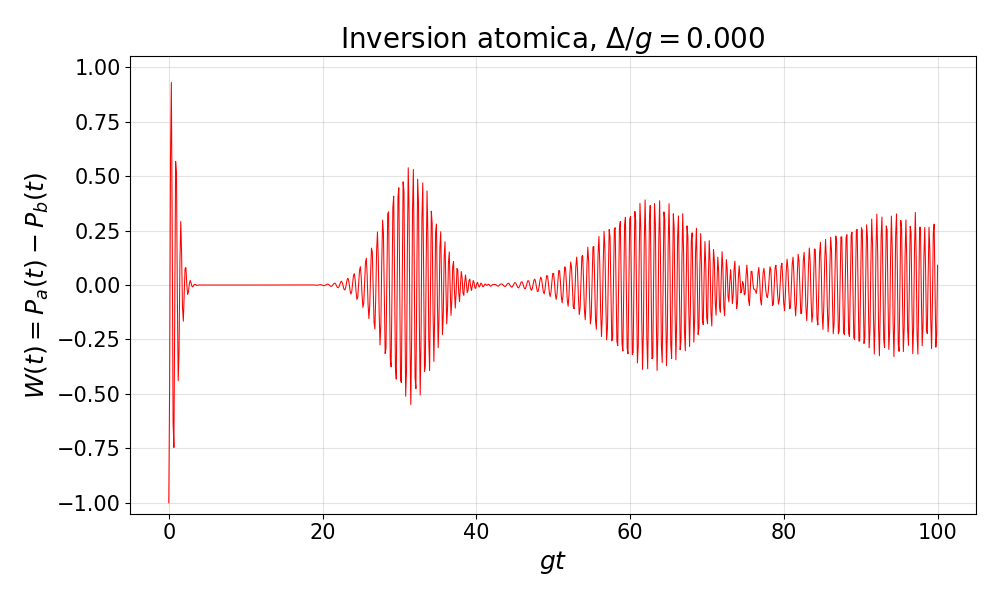
\includegraphics[width=0.86\linewidth]{../../notas-doctorado/imgs/inversion_base.png}
  \caption{Inversi\'on at\'omica en resonancia para un \'atomo inicialmente en
  $\ket{b}$ y un campo coherente con $\bar n=25$.}
\end{figure}

Para ver de d\'onde sale la escala temporal del revival, se escribe
\begin{equation}
  n=\bar n+m,
\end{equation}
y se expande la ra\'iz alrededor de $\bar n$:
\begin{equation}
  \sqrt{\bar n+m}
  =
  \sqrt{\bar n}
  +
  \frac{m}{2\sqrt{\bar n}}
  -
  \frac{m^2}{8\bar n^{3/2}}
  +\cdots .
\end{equation}
Por tanto, la fase que aparece en la inversi\'on se aproxima por
\begin{equation}
  2gt\sqrt{\bar n+m}
  \simeq
  2gt\sqrt{\bar n}
  +
  \frac{gt}{\sqrt{\bar n}}m
  -
  \frac{gt}{4\bar n^{3/2}}m^2+\cdots .
\end{equation}
El t\'ermino lineal controla la realineaci\'on de fases entre componentes
vecinas. Cuando su incremento es $2\pi$, los sectores cercanos al m\'aximo de
la distribuci\'on vuelven a estar aproximadamente en fase:
\begin{equation}
  \frac{gT_R}{\sqrt{\bar n}}\simeq 2\pi,
  \qquad
  T_R\simeq \frac{2\pi\sqrt{\bar n}}{g}.
\end{equation}
En la convenci\'on usada para la figura, la escala se toma con
$\sqrt{\bar n+1}$, de modo que para $\bar n=25$ se obtiene
\begin{equation}
  gT_R=2\pi\sqrt{26}\simeq 32.038.
\end{equation}
El t\'ermino cuadr\'atico no permite una realineaci\'on perfecta: corrige la
fase, ensancha los revivals y, a tiempos m\'as largos, favorece revivals
fraccionarios.

Tambi\'en es \'util introducir la se\~nal compleja
\begin{equation}
  S(t)=\sum_{n=0}^{\infty}P_n\ee^{\ii 2gt\sqrt{n}},
\end{equation}
de modo que
\begin{equation}
  I(t)=-\Real S(t).
\end{equation}
El m\'odulo de $S(t)$ mide qu\'e tan sincronizadas est\'an las contribuciones
de los distintos sectores de fotones. Cuando $|S(t)|$ es grande, aparece una
oscilaci\'on visible; cuando $|S(t)|$ es peque\~no, las contribuciones se
cancelan y la inversi\'on colapsa hacia cero.

\section{Funci\'on Q de Husimi del campo}

La din\'amica anterior tambi\'en deja una huella directa en el estado reducido
del campo. Si el \'atomo no se mide, el campo se describe por
\begin{equation}
  \hat\rho_{\mathrm{c}}(t)
  =
  \Tr_{\mathrm{at}}
  \left[
  \ket{\psi(t)}\bra{\psi(t)}
  \right].
\end{equation}
Para el \'atomo inicialmente en $\ket{b}$,
\begin{equation}
  \ket{\psi(t)}
  =
  \sum_{n=0}^{\infty}W_n
  \left[
  \cos(gt\sqrt{n})\ket{b,n}
  -
  \ii\sin(gt\sqrt{n})\ket{a,n-1}
  \right],
\end{equation}
y al trazar sobre el \'atomo se obtiene una mezcla de dos contribuciones de
campo:
\begin{equation}
  \hat\rho_{\mathrm{c}}(t)
  =
  \ket{\phi_b(t)}\bra{\phi_b(t)}
  +
  \ket{\phi_a(t)}\bra{\phi_a(t)},
\end{equation}
con
\begin{equation}
  \ket{\phi_b(t)}
  =
  \sum_{n=0}^{\infty}W_n\cos(gt\sqrt{n})\ket{n},
\end{equation}
\begin{equation}
  \ket{\phi_a(t)}
  =
  -\ii\sum_{n=1}^{\infty}W_n\sin(gt\sqrt{n})\ket{n-1}.
\end{equation}
La funci\'on Q de Husimi se define como
\begin{equation}
  \boxed{
  Q(\beta,t)
  =
  \frac{1}{\pi}
  \bra{\beta}\hat\rho_{\mathrm{c}}(t)\ket{\beta}.
  }
\end{equation}
Sustituyendo la descomposici\'on anterior,
\begin{equation}
  Q(\beta,t)
  =
  \frac{1}{\pi}
  \left(
  |\braket{\beta|\phi_b(t)}|^2
  +
  |\braket{\beta|\phi_a(t)}|^2
  \right).
\end{equation}
Esta representaci\'on en espacio de fase permite ver c\'omo el paquete
coherente inicial se deforma, se separa en componentes y vuelve a reagruparse
alrededor de los tiempos de revival.

\begin{figure}[htbp]
  \centering
  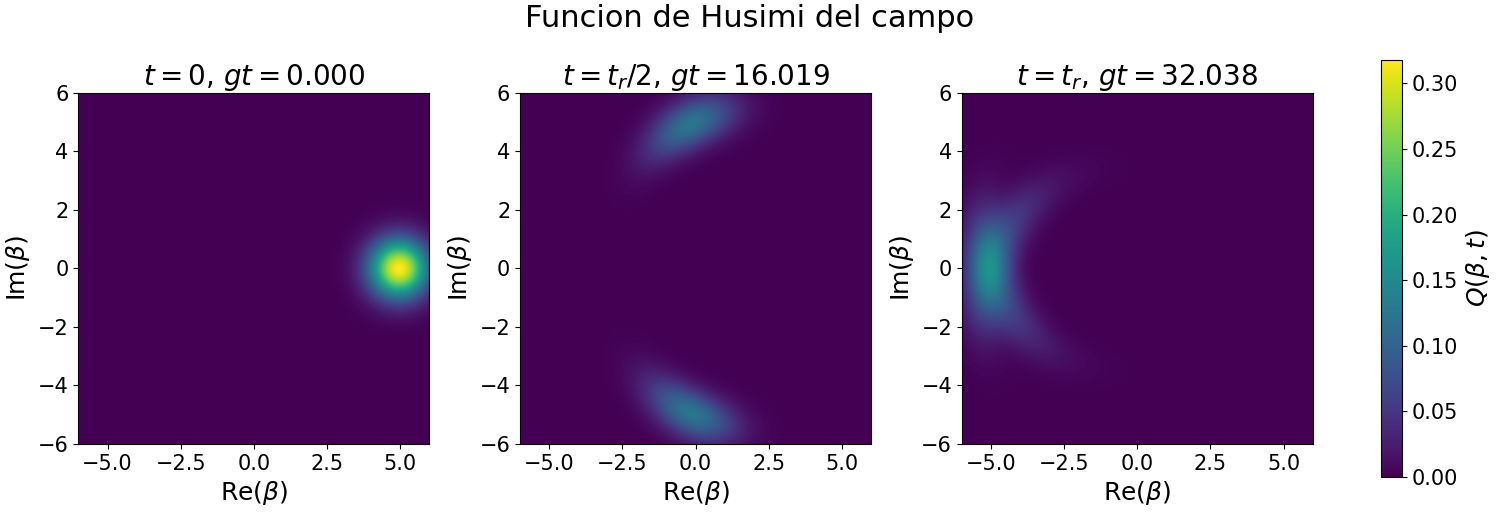
\includegraphics[width=\linewidth]{../../notas-doctorado/imgs/Q_base.png}
  \caption{Funci\'on Q de Husimi del campo para $\bar n=25$ en $t=0$,
  $t=T_R/2$ y $t=T_R$.}
\end{figure}

\section{Preparaci\'on de superposiciones coherentes}

Una aplicaci\'on importante del entrelazamiento \'atomo-campo es la
preparaci\'on de superposiciones de estados coherentes con fases distintas, es
decir, estados tipo gato. Se considera un \'atomo preparado en
\begin{equation}
  \ket{\psi_{\mathrm{at}}(0)}
  =
  C_a\ket{a}+C_b\ket{b},
\end{equation}
y un campo
\begin{equation}
  \ket{\psi_{\mathrm{c}}(0)}
  =
  \sum_{n=0}^{\infty}W_n\ket{n}.
\end{equation}
En el r\'egimen altamente desintonizado, el intercambio real de excitaciones
queda suprimido, pero el campo adquiere fases condicionadas al estado
at\'omico. Por eso la evoluci\'on tiene la forma
\begin{equation}
  \ket{\psi(t)}
  =
  \sum_{n=0}^{\infty}W_n
  \left[
  C_a\ee^{\ii\phi_{a,n}(t)}\ket{a,n}
  +
  C_b\ee^{\ii\phi_{b,n}(t)}\ket{b,n}
  \right].
\end{equation}
En el l\'imite dispersivo las fases son lineales en el n\'umero de fotones,
m\'as fases globales:
\begin{equation}
  \phi_{a,n}(t)=\phi_a(t)+n\theta_a(t),
  \qquad
  \phi_{b,n}(t)=\phi_b(t)+n\theta_b(t),
\end{equation}
con $\theta_{a,b}(t)$ proporcionales a $g^2t/\Delta$. Esto significa que cada
componente at\'omica rota el estado del campo en una direcci\'on distinta en el
espacio de fase.

Si ahora se mide el \'atomo y se acepta \'unicamente el resultado
\begin{equation}
  \ket{F_{\mathrm{at}}}=f_a\ket{a}+f_b\ket{b},
\end{equation}
el estado condicionado del campo es
\begin{equation}
  \boxed{
  \ket{\psi_{\mathrm{c}}(t;F_{\mathrm{at}})}
  =
  \mathcal N
  \sum_{n=0}^{\infty}W_n
  \left[
  f_a^*C_a\ee^{\ii\phi_{a,n}(t)}
  +
  f_b^*C_b\ee^{\ii\phi_{b,n}(t)}
  \right]\ket{n}.
  }
\end{equation}
La constante $\mathcal N$ normaliza el estado y contiene la probabilidad de
\'exito de la postselecci\'on. Lo esencial es que las amplitudes originales
$W_n$ no solo se multiplican por n\'umeros constantes: reciben fases
dependientes de $n$. Por eso la medici\'on at\'omica puede cambiar
considerablemente el estado del campo.

Si el campo inicial es coherente,
\begin{equation}
  \ket{\alpha}
  =
  \ee^{-|\alpha|^2/2}
  \sum_{n=0}^{\infty}
  \frac{\alpha^n}{\sqrt{n!}}\ket{n},
\end{equation}
entonces multiplicar cada amplitud por $\ee^{\ii n\theta}$ equivale a rotar la
amplitud coherente:
\begin{equation}
  \ee^{\ii n\theta}\alpha^n
  =
  \left(\alpha\ee^{\ii\theta}\right)^n.
\end{equation}
As\'i, despu\'es de la proyecci\'on at\'omica,
\begin{equation}
  \boxed{
  \ket{\psi_{\mathrm{c}}}
  \propto
  A\ket{\alpha\ee^{\ii\theta_a}}
  +
  B\ket{\alpha\ee^{\ii\theta_b}},
  }
\end{equation}
donde $A=f_a^*C_a\ee^{\ii\phi_a}$ y $B=f_b^*C_b\ee^{\ii\phi_b}$. Esta es una
superposici\'on coherente de dos paquetes con fases diferentes. Cuando las dos
amplitudes quedan bien separadas en espacio de fase, el estado preparado es el
estado gato discutido en las notas de estados apachurrados.

\section{Ingenier\'ia de estados finitos de Fock}

El objetivo ahora es preparar un estado finito del campo,
\begin{equation}
  \ket{\psi_{\mathrm{target}}}
  =
  \sum_{n=0}^{N}d_n\ket{n}
  =
  d_0\ket{0}+d_1\ket{1}+\cdots+d_N\ket{N}.
\end{equation}
Como se parte del vac\'io, para llegar a $\ket{N}$ se deben transferir
excitaciones a la cavidad. Una idea b\'asica ser\'ia inyectar $N$ \'atomos
excitados y hacer que todos salgan en el estado base; de esta forma cada
\'atomo depositar\'ia una excitaci\'on en el campo. Sin embargo, eso solo
produce transferencia de energ\'ia. Para preparar una superposici\'on coherente
de los primeros $N+1$ estados de Fock, tambi\'en se necesita controlar las
fases y las interferencias entre los distintos caminos.

El procedimiento consiste en enviar \'atomos resonantes, uno por uno. El
$k$-\'esimo \'atomo entra en una superposici\'on
\begin{equation}
  \ket{\chi_k}
  =
  \alpha_k\ket{a}
  +
  \beta_k\ket{b},
\end{equation}
interact\'ua durante un tiempo $\tau_k$ y luego se mide. Se conservan solo las
corridas en las que el \'atomo sale en $\ket{b}$. Si antes del \'atomo $k$ el
campo est\'a en
\begin{equation}
  \ket{\psi_{\mathrm{c}}^{(k-1)}}
  =
  \sum_{n=0}^{k-1}c_n^{(k-1)}\ket{n},
\end{equation}
entonces, despu\'es de la interacci\'on resonante y de postseleccionar el
\'atomo en $\ket{b}$, los nuevos coeficientes no normalizados cumplen la
recurrencia
\begin{equation}
  \boxed{
  c_n^{(k)}
  =
  \beta_k\cos(g\tau_k\sqrt{n})\,c_n^{(k-1)}
  -
  \ii\alpha_k\sin(g\tau_k\sqrt{n})\,c_{n-1}^{(k-1)},
  }
\end{equation}
con $c_{-1}^{(k-1)}=0$. El primer t\'ermino corresponde al camino donde el
\'atomo entr\'o en $\ket{b}$ y no deposit\'o excitaci\'on en la cavidad. El
segundo t\'ermino corresponde al camino donde el \'atomo entr\'o en $\ket{a}$,
emiti\'o un fot\'on y sali\'o en $\ket{b}$. La misma amplitud final $\ket{n}$
puede recibir contribuciones de dos historias distintas; por eso aparece
interferencia.

Para el primer \'atomo, con la cavidad inicialmente en el vac\'io,
$c_0^{(0)}=1$, se obtiene
\begin{equation}
  \ket{\tilde\psi_{\mathrm{c}}^{(1)}}
  =
  \beta_1\ket{0}
  -
  \ii\alpha_1\sin(g\tau_1)\ket{1}.
\end{equation}
Despu\'es de normalizar, el campo queda en una superposici\'on de $\ket{0}$ y
$\ket{1}$. Para el segundo \'atomo,
\begin{equation}
  \ket{\tilde\psi_{\mathrm{c}}^{(2)}}
  =
  c_0^{(2)}\ket{0}
  +
  c_1^{(2)}\ket{1}
  +
  c_2^{(2)}\ket{2}.
\end{equation}
Solo hay un camino que lleva de $\ket{0}$ a $\ket{2}$: los dos \'atomos deben
transferir su excitaci\'on. Tambi\'en hay un camino que deja el vac\'io sin
alterar: ambos \'atomos deben contribuir por su componente $\ket{b}$. En
cambio, para terminar en $\ket{1}$ hay dos caminos indistinguibles: puede haber
emitido el primer \'atomo o puede haber emitido el segundo. La amplitud final
de $\ket{1}$ es la suma coherente de ambos caminos.

Repitiendo el proceso con $N$ \'atomos, cada paso agrega como m\'aximo un
fot\'on y aumenta en una unidad la dimensi\'on accesible del espacio de Fock.
Al escoger las amplitudes $\alpha_k,\beta_k$ y los tiempos $\tau_k$, se pueden
ajustar los coeficientes finales para aproximar o realizar exactamente el
conjunto deseado $\{d_0,d_1,\ldots,d_N\}$, siempre condicionado a que todas las
mediciones at\'omicas den el resultado postseleccionado.

\bigskip

La idea que unifica toda la nota es que la medici\'on no es solo lectura. En
un sistema entrelazado, proyectar el \'atomo selecciona una rama coherente del
campo; por eso una secuencia controlada de interacciones y mediciones puede
usarse como herramienta de preparaci\'on de estados.

\end{document}
